\documentclass[12pt]{article}

\usepackage[utf8]{inputenc}
\usepackage[T1]{fontenc}
\usepackage[ngerman]{babel}
\usepackage[ngerman=ngerman-x-latest]{hyphsubst}
\usepackage{csquotes}
\usepackage{hyphenat}
\usepackage{textcmds}
\usepackage{xspace}
\usepackage{amsmath}
\usepackage{amsfonts}
\usepackage{mathtools}
\usepackage{authblk}
\usepackage{svg}
\usepackage{lipsum}
\usepackage{subcaption}
\usepackage{pdfpages}
\usepackage[printonlyused]{acronym}
\usepackage{framed}
\usepackage{tikz}
\usepackage{pgfplots}

\usepackage{float}
\usepackage[section]{placeins}
\usepackage{wrapfig}
\newfloat{floatingequation}{htbp}{loe}
\floatname{floatingequation}{Gleichung}
\newcommand{\floatingequationautorefname}{Gleichung}

\usepackage{geometry}
\geometry{a4paper, margin=1in}

\usepackage{graphicx}
\usepackage{chngpage}
\usepackage{calc}

\usepackage{hyperref}
\hypersetup{
    colorlinks=true,
    linkcolor=black,
    filecolor=blue,
    urlcolor=blue,
    pdftitle={Bachelorarbeit},
    pdfauthor={Nik Benson},
    pdfpagemode=FullScreen,
}
\urlstyle{same}

\usepackage{xcolor}
\definecolor{codegreen}{rgb}{0,0.6,0}
\definecolor{codegray}{rgb}{0.5,0.5,0.5}
\definecolor{codepurple}{rgb}{0.58,0,0.82}
\definecolor{backcolour}{rgb}{0.95, 0.95, 0.96}
\definecolor{app_repo_color}{rgb}{0.98, 0.89, 0.80}

\PassOptionsToPackage{dvipsnames}{xcolor}
\usepackage{listings}
\lstdefinelanguage{Kotlin}{
    sensitive=true,
    comment=[l]{//},
    morecomment=[s]{/*}{*/},
    morestring=[b]",
    morestring=[s]{"""*}{*"""},
    keywords={!in, !is, abstract, actual, annotation, as, as?, break, by, catch, class, companion, const, constructor, continue, crossinline, data, delegate, do, dynamic, else, enum, expect, external, false, field, file, final, finally, for, fun, get, if, import, in, infix, init, inline, inner, interface, internal, is, lateinit, noinline, null, object, open, operator, out, override, package, param, private, property, protected, public, receiveris, reified, return, return@, sealed, set, setparam, super, suspend, tailrec, this, throw, true, try, typealias, typeof, val, var, vararg, when, where, while},
    ndkeywords={@Deprecated, @JvmField, @JvmName, @JvmOverloads, @JvmStatic, @JvmSynthetic, Array, Byte, Double, Float, Int, Integer, Iterable, Long, Runnable, Short, String, Any, Unit, Nothing},
    emph={filter, first, firstOrNull, forEach, lazy, map, mapNotNull, println},
    commentstyle={\color{codegreen}\ttfamily},
    stringstyle={\color{codepurple}\ttfamily},
    keywordstyle={\color{magenta}\bfseries},
    ndkeywordstyle={\color{orange}\bfseries},
    emphstyle={\color{codepurple}},
    identifierstyle=\color{black},
}
\lstdefinelanguage{Dart}{
    sensitive=true,
    comment=[l]{//},
    morecomment=[s]{/*}{*/},
    morestring=[b]',
    morestring=[b]",
    morestring=[s]{'''*}{*'''},
    morestring=[s]{"""*}{*"""},
    keywords={abstract, as, assert, async, await, base, break, case, catch, class, const, continue, covariant, default, deferred, do, dynamic, else, enum, export, extends, extension, external, factory, false, final, finally, for, Function, get, if, implements, import, in, interface, is, late, library, mixin, new, null, on, operator, part, required, rethrow, return, sealed, set, show, static, super, switch, sync, this, throw, true, try, typedef, var, void, when, while, with, yield},
    ndkeywords={int, double, String, bool, List, Set, Map, Never, Null, Object, Enum, Future, Iterable},
    emph={},
    commentstyle={\color{codegreen}\ttfamily},
    stringstyle={\color{codepurple}\ttfamily},
    keywordstyle={\color{magenta}\bfseries},
    ndkeywordstyle={\color{orange}\bfseries},
    emphstyle={\color{codepurple}},
    identifierstyle=\color{black},
}
\lstdefinelanguage{DesignSystem}{
    sensitive=true,
    comment=[l]{//},
    morecomment=[s]{/*}{*/},
    morestring=[b]",
    keywords={abstract, by, switch, if},
    ndkeywords={PrimitiveTokens, PrimitiveTokensSet, DesignSystem, subsystems, properties, tokens, resolve, primitive, app},
    emph={Color, Brightness, ButtonState, FontWeight, String},
    commentstyle={\color{codegreen}\ttfamily},
    stringstyle={\color{codepurple}\ttfamily},
    keywordstyle={\color{magenta}\bfseries},
    ndkeywordstyle={\color{orange}\bfseries},
    emphstyle={\color{codepurple}},
    identifierstyle=\color{black},
}
\lstdefinelanguage{PlayerConfig}{
    sensitive=true,
    morecomment=[s]{<}{>},
    commentstyle={\color{codegreen}\ttfamily},
    stringstyle={\color{codepurple}\ttfamily},
    keywordstyle={\color{magenta}\bfseries},
    ndkeywordstyle={\color{orange}\bfseries},
    emphstyle={\color{codepurple}},
    identifierstyle=\color{black},
}
\lstdefinelanguage{txt}{
    commentstyle={\color{codegreen}\ttfamily},
    stringstyle={\color{codepurple}\ttfamily},
    keywordstyle={\color{magenta}\bfseries},
    ndkeywordstyle={\color{orange}\bfseries},
    emphstyle={\color{codepurple}},
    identifierstyle=\color{black},
}
\lstdefinelanguage{JavaScript}{
    sensitive=false,
    keywords={typeof, new, true, false, catch, function, return, null, catch, switch, var, if, in, while, do, else, case, break},
    ndkeywords={class, export, boolean, throw, implements, import, this},
    identifierstyle=\color{black},
    comment=[l]{//},
    morecomment=[s]{/*}{*/},
    morestring=[b]',
    morestring=[b]",
    commentstyle={\color{codegreen}\ttfamily},
    stringstyle={\color{codepurple}\ttfamily},
    keywordstyle={\color{magenta}\bfseries},
    ndkeywordstyle={\color{orange}\bfseries},
    emphstyle={\color{codepurple}},
    identifierstyle=\color{black},
}
\lstdefinelanguage{tokens}{
    sensitive=true,
    comment=[l]{//},
    morecomment=[s]{/*}{*/},
    morestring=[b]",
    keywords={},
    ndkeywords={QUESTION_1, QUESTION_2, QUESTION_3, BOOL, FLOAT},
    emph={},
    commentstyle={\color{codegreen}\ttfamily},
    stringstyle={\color{codepurple}\ttfamily},
    keywordstyle={\color{magenta}\bfseries},
    ndkeywordstyle={\color{orange}\bfseries},
    emphstyle={\color{codepurple}},
    identifierstyle=\color{black},
}
\lstdefinelanguage{c}{
    sensitive=true,
    comment=[l]{//},
    morecomment=[s]{/*}{*/},
    morestring=[b]",
    keywords={auto, break, case, char, const, continue, default, do, double, else, enum, extern, float, for, goto, if, int, long, register, return, short, signed, sizeof, static, struct, switch, typedef, union, unsigned, void, volatile, while},
    ndkeywords={NULL, TRUE, FALSE, EOF},
    emph={printf, scanf, malloc, free, memcpy, strcmp},
    commentstyle={\color{codegreen}\ttfamily},
    stringstyle={\color{codepurple}\ttfamily},
    keywordstyle={\color{magenta}\bfseries},
    ndkeywordstyle={\color{orange}\bfseries},
    emphstyle={\color{codepurple}},
    identifierstyle=\color{black},
}

\lstdefinelanguage{yacc}{
    sensitive=true,
    comment=[l]{//},
    morecomment=[s]{/*}{*/},
    morestring=[b]",
    keywords={token, precedence, nonterminal, start, \%\%},
    ndkeywords={\$\$, \$1, \$2, \$3, \$4, \$5, accept, error},
    emph={yylex, yyparse, yylval, yytext, YYSTYPE},
    commentstyle={\color{codegreen}\ttfamily},
    stringstyle={\color{codepurple}\ttfamily},
    keywordstyle={\color{magenta}\bfseries},
    ndkeywordstyle={\color{orange}\bfseries},
    emphstyle={\color{codepurple}},
    identifierstyle=\color{black},
}

\lstdefinelanguage{lex}{
    sensitive=true,
    comment=[l]{//},
    morecomment=[s]{/*}{*/},
    morestring=[b]",
    keywords={BEGIN, DEF, RETURN, RULE},
    ndkeywords={yylval, yytext, ECHO, yyleng},
    emph={yylex, yyerror, input},
    commentstyle={\color{codegreen}\ttfamily},
    stringstyle={\color{codepurple}\ttfamily},
    keywordstyle={\color{magenta}\bfseries},
    ndkeywordstyle={\color{orange}\bfseries},
    emphstyle={\color{codepurple}},
    identifierstyle=\color{black},
}
\lstdefinelanguage{mps-concept}{
    sensitive=true,
    morecomment=[s]{<}{>},
    morecomment=[s]{<<}{>>},
    morestring=[b]",
    keywords={BaseConcept},
    ndkeywords={abstract, concept, extends, implements, instance, can, be, root, alias, short, description, properties, children, references},
    emph={true, false},
    commentstyle={\color{codegreen}\ttfamily},
    stringstyle={\color{codepurple}\ttfamily},
    keywordstyle={\color{magenta}\bfseries},
    ndkeywordstyle={\color{orange}\bfseries},
    emphstyle={\color{codepurple}},
    identifierstyle=\color{black},
}


\lstdefinestyle{default}{
    backgroundcolor=\color{backcolour},
    commentstyle=\color{codegreen},
    keywordstyle=\color{orange},
    numberstyle=\tiny\color{codegray},
    stringstyle=\color{codepurple},
    basicstyle=\ttfamily\footnotesize,
    breakatwhitespace=false,
    breaklines=true,
    captionpos=b,
    keepspaces=true,
    numbers=left,
    numbersep=5pt,
    showspaces=false,
    showstringspaces=false,
    showtabs=false,
    tabsize=2,
}

\lstset{style=default}

\renewcommand{\lstlistingname}{Code}
\renewcommand{\lstlistlistingname}{Codeverzeichnis}

\DeclarePairedDelimiter\ceil{\lceil}{\rceil}
\DeclarePairedDelimiter\floor{\lfloor}{\rfloor}

\title{Prototyp zur Verwendung von Domain Specific Languages (DSL) zur einfachen und präzisen Beschreibung von Constraints in Logik und UI}
\author{Nik Benson}
\affil{\href{mailto:nik.benson@studmail.w-hs.de}{nik.benson@studmail.w-hs.de}}


\usepackage[backend=biber, style=iso-authoryear]{biblatex}
\bibliography{main}

\begin{document}
    \pagenumbering{gobble}
\begin{titlepage}
    \maketitle
    \vspace*{\fill}
    \begin{flushleft}
        \includesvg[width={0.6\textwidth}]{../assets/img/logos/nettrek}
    \end{flushleft}
    \vspace{1cm}
    \begin{flushright}
        
\includegraphics[width={0.6\textwidth}]{../assets/img/logos/whs}
    \end{flushright}
    \vspace*{\fill}
    \begin{large}
        \begin{tabular}{r l}
            \textbf{Betrieb:}     & netTrek GmbH \& Co. KG         \\
            \textbf{Institution:} & Westfälische Hochschule        \\
            \textbf{Erstprüfer:}  & Prof.~Dr.--~Ing.~Martin Guddat \\
            \textbf{Zweitprüfer}  & B.~Sc.~Ali~Kortak              \\
        \end{tabular}
    \end{large}
\end{titlepage}

    \pagenumbering{Roman}
\setcounter{page}{2}
\tableofcontents
\addcontentsline{toc}{section}{Abbildungsverzeichnis}
\listoffigures
\addcontentsline{toc}{section}{Tabellenverzeichnis}
\listoftables
\addcontentsline{toc}{section}{Codeverzeichnis}
\lstlistoflistings
\newpage
\addcontentsline{toc}{section}{Abkürzungsverzeichnis}
\section*{Abkürzungsverzeichnis}
\begin{acronym}[POSIX]
    \acro{AST}{Abstract Syntax Tree}

    \acro{CFG}{context--free grammar}

    \acro{CLI}{Comand Line Interface}
    \acroplural{CLI}[CLI]{Comand Line Interfaces}

    \acro{DBMS}{Database Management System}
    \acroplural{DBMS}[DBMS]{Database Management Systems}

    \acro{DSL}{Domain--Specific Language}
    \acroplural{DSL}[DSL]{Domain--Specific Languages}

    \acro{GCC}{GNU Compiler Collection}

    \acro{GPL}{General--Purpose Language}
    \acroplural{GPL}[GPL]{General--Purpose Languages}

    \acro{ISO}{International Organization for Standardization}

    \acro{IDE}{Integrated Development Environment}

    \acro{IT}{Information Technology}

    \acro{JSON}{JavaScript Object Notation}

    \acro{LALR}{lookahead left-to-right}

    \acro{LLM}{Large Language Model}
    \acroplural{LLM}[LLM]{Large Language Models}

    \acro{LLVM}{Low Level Virtual Machine}

    \acro{MPS}{Meta Programming System}

    \acro{POSIX}{Portable Operating System Interface}

    \acro{RegEx}{Regular Expression}
    \acroplural{RegEx}[RegEx]{Regular Expressions}

    \acro{SQL}{Structured Query Language}

    \acro{UI}{User Interface}
    \acroplural{UI}[UI]{User Interfaces}

    \acro{YACC}{Yet Another Compiler Compiler}
\end{acronym}
\newpage
\pagenumbering{arabic}

    % 1 : 2
    % 2 : 15?
    % 3 : 6?
    % 4 : 10?
    % 5 : 2?
    % 6 : 3?
    % 7 : 2?
    % * = 35


    \section{Einleitung}\label{sec:einleitung}
    In dieser Arbeit soll evaluiert werden, ob das Entwickeln von \acp{DSL} mit modernen Tools wirtschaftlich ist.

\subsection{Motivation}\label{subsec:motivation}
In den vergangenen Jahren ist das, was mittels Software möglich ist stark angestiegen.
Damit wachsen auch immer mehr die Anforderungen an Entwickler.
Einen Teil der Last wird dabei schon seit einiger Zeit versucht durch Low-- bzw.\ No--Code--Solutions zu umgehen.
Ein gutes Beispiel sind dabei die Menge an neuen Website--Baukästen, die zuletzt beworben wurden. \autocite{p-2024}

Mit besonders großem Erfolg werden dabei Systeme beworben, die auf spezifische Bereiche spezialisiert sind.
Beispiele wären zum Beispiel die aktuell vom DSB geförderte Vereinswebsite~\autocite{deutscher-olympischer-sportbund-ev-no-date} sowie die beiden E-Commerce Plattformen Shopware~\autocite{ag-no-date} und Shopify~\autocite{shopify-international-ltd-no-date}.

Daraus folgt die Annahme, dass das notwendige Expertenwissen zur inbetriebnahme von Systemen weiterhin gewünscht ist.
Lediglich das Expertenwissen zur Softwareentwicklung sollte reduziert werden.

Eine allgemeingültige lösung wollen aktuell \acp{LLM} schaffen.
Diesen mangelt es allerdings für viele Anwendungsfälle an Präzision.

\acp{DSL} bieten hier eine potenzielle Lösung.

\subsubsection{Aktuelle Herausforderungen}
Die Entwicklung von \acp{DSL} ist jedoch nach wie vor mit einigen Herausforderungen verbunden.
Dazu gehört die hohe Komplexität der \ac{DSL}--Entwicklung, die tiefgreifendes Wissen in Sprachtheorie, Compilerbau und Softwareentwicklung erfordert.
Es fehlt zudem an einem einheitlichen Ansatz zur Entwicklung von \acp{DSL}, der für verschiedene Anwendungsbereiche geeignet ist.
Des Weiteren sind \acp{DSL} oft nicht in bestehende Entwicklungsumgebungen integriert, was zu Inkompatibilitäten und Fragmentierung führt.

\subsubsection{Bedarf an intuitiven und effizienten \acp{DSL}}
Eine Bedarfsanalyse kann diese Arbeit leider nicht bieten, allerdings soll sie die Möglichkeiten aufzeigen.

Sprachen schnell formulieren zu können hat in jedem Fall viele Anwendungsmöglichkeiten, die aktuell weitestgehend mittels anderer technologien gelöst werden.

Häufig kommen im Enterprise Bereich hier komplizierte \acp{UI} zum Einsatz.
Ein Beispiel dafür wäre SAP\@. % TODO: Quelle hinzufügen
Hier wurde sich dafür entschieden eine parallele zwischen \acp{UI} und \acp{DSL} zu nutzen, da \ac{DSL} ab einer gewissen komplexität einfacher zu handhaben sind.

Wir nehmen an, dass der Bedarf aktuell künstlich durch weniger optimale Technologien gedeckt wird, da \acp{DSL} zu kompliziert sind.
Es ist davon auszugehen, dass \ac{DSL} wieder inder Breite eingesetzt werden, sobald die Technologie dafür hinreichend einfach zu lernen ist.

\subsubsection{Potenzial des Prototyps}
Der vorliegende Prototyp zielt darauf ab zu prüfen, ob \ac{MPS}~\autocite{jetbrains-sro-2021} die Entwicklung von \acp{DSL} bereits so weit vereinfacht hat, dass es wirtschaftlich ist, diese Technologie einzusetzen.

Des weiteren soll die Interaktion zwischen Entwicklern und Designern in dem später erläuterten konkreten Beispiel optimiert werden.
Dabei werden unnötige Copy--Paste Arbeiten unterbunden.
Der konkrete Anwendungsfall ist allerdings in dieser Arbeit zweitrangig.

\subsubsection{Persönliche Motivation}
Die Entwicklung des Prototyps ist von meiner persönlichen Motivation geleitet, die Potenziale von \acp{DSL} zu erschließen und die Entwicklung von Software zu verbessern.
Ich sehe \acp{DSL} als eine Möglichkeit, auch Laien die präzise Beschreibung von komplexen Systemen zu ermöglichen und die IT-Branche zu demokratisieren.
Durch die Förderung der \ac{DSL}--Entwicklung und die Verbreitung von Wissen über diese Technologie möchte ich zu einer Renaissance des Compilerbaus beitragen und die Wertschätzung für die Grundlagen der Softwareentwicklung stärken.

\subsection{Zielsetzung}\label{subsec:zielsetzung}
\lipsum[5]

\subsection{Aufbau der Arbeit}\label{subsec:aufbau-der-arbeit}
\lipsum[5]



    \section{Grundlagen}\label{sec:grundlagen}
    In diesem Kapitel werden die grundsätzlichen Definitionen und eine historische einordnung sowie ein Überblich über die aktuellen Möglichkeiten von \ac{DSL} geschaffen.

\subsection{\aclp{DSL}}\label{subsec:domain-specific-languages}
Die erste Frage, die es zu klären gibt, ist: Was sind eigentlich \ac{DSL}?
\begin{displayquote}[\cite{jetbrains-sro-no-dateC}]
    A \ac{DSL} is a programming language with a higher level of abstraction optimized for a specific class of problems.
    A \ac{DSL} uses the concepts and rules from the field or domain.
\end{displayquote}
Laut JetBrains definieren sich \acp{DSL} also über ihr Sprachdesign, welches Konzepte einer spezifischen, fachlichen Domäne beinhaltet.
Wikipedia definiert es etwas anders:
\begin{displayquote}[\cite{wikipedia-contributors-2024C}]
    A \ac{DSL} is a computer language specialized to a particular application domain.
    This is in contrast to a \ac{GPL}, which is broadly applicable across domains.
\end{displayquote}
Hier werden \acp{DSL} als gegenteil von \acp{GPL} genannt, welche zusammen die Programmiersprachen ausmachen.
Diese sind im Wörterbuch definiert als:
\begin{displayquote}[\cite{unknown-author-no-date}]
    Code of reserved words and symbols used in computer programs, which give instructions to the computer on how to accomplish certain computing tasks.
\end{displayquote}
Also eine Kodierung, welche Anweisungen an einen Computer gibt.

Zusammenfassend lässt sich sagen, dass \acp{DSL} Kodierungen sind, die fachspezifisch von einer Menge von Schlüsselwörtern und strukturierten, dynamischen Inhalt auf eine von (mindestens) einem Computer--(Programm) verstandene Eingabe--(Datei) abbildet.
Dabei stehen fachspezifische Paradigmen vor den klassischen Programmierparadigmen~\autocite{wikipedia-contributors-2024D} im Zentrum des Sprachdesigns.

Das wohl bekannteste Beispiel ist \ac{SQL}.~\autocite{unknown-author-2023}
\ac{SQL} ist eine durch die \ac{ISO} genormte \ac{DSL}; spezifischer eine sogenannte \textit{query language}.
Auf Deutsch Abfragesprachen genannt, dienen diese \acp{DSL}, der interaktionen mit \acp{DBMS}.
Die Domäne ist in diesem Fall also die Datenhaltung \textit{strukturierter} Daten.

Da es etliche \acp{DBMS} gibt, welche dem \ac{SQL}--Standard folgen, gibt es für \ac{SQL} auch etliche Compiler--Pipelines beziehungsweise Interpreter.
Diese Compiler--Pipelines sind dabei stark mit dem jeweiligen \ac{DBMS} verwoben.
Es gibt also keine einheitliche Codebasis.
Dies wäre mit bekannten Tools des Compilerbaus, namentlich \textbf{Lex} \& \textbf{YACC}.
Diese werden im folgenden Kapitel behandelt.

\begin{figure}[ht]
    \begin{subfigure}[c]{0.5\textwidth}
        \begin{center}
            \includegraphics[height=2.5cm]{../assets/img/diagrams/compiler.mmd}
        \end{center}
        \caption{Compiler}
        \label{subfig:compiler-and-interpreter-compiler}
    \end{subfigure}
    \begin{subfigure}[c]{0.5\textwidth}
        \begin{center}
            \includegraphics[height=2.5cm]{../assets/img/diagrams/interpreter.mmd}
        \end{center}
        \caption{Interpreter}
        \label{subfig:compiler-and-interpreter-interpreter}
    \end{subfigure}
    \caption{Compiler \& Interpreter~\autocite{aho-2006}}
    \label{fig:compiler-and-interpreter}
\end{figure}
\newpage

\subsection{Compilerbau}\label{subsec:compilerbau}
\begin{wrapfigure}{rH}{0.47\textwidth}
    \begin{center}
        \includegraphics[width=0.45\textwidth]{../assets/img/diagrams/compiler_phases.mmd}
    \end{center}
    \caption{Phasen der Compiler--Pipeline~\autocite{aho-2006}}
    \label{fig:compiler-phases}
\end{wrapfigure}
Was von Entwicklern umgangssprachlich \qq{Compiler} genannt wird, bezeichnet eigentlich die Compiler--Pipeline.
Der eigentliche Compiler, oder auch Code Generator, (Siehe \autoref{fig:compiler-phases}) ist ein Tool, welches aus einer abstrakten Representation die Zielsprache, im folgenden Programm genannt, generiert.

Ein Programm ist dabei definiert als eine \qq{Black--Box}, welche eine Eingabe in eine Ausgabe transformiert.
Damit kann zwischen zwei verschiedenen Aufbauten unterscheiden: Compiler erstellen aus Code ein Programm, welches eine Eingabe in eine Ausgabe transformiert (Siehe \autoref{subfig:compiler-and-interpreter-compiler}) und Interpreter transformieren unter der Verwendung von Code eine Eingabe in eine Ausgabe.~(Siehe \autoref{subfig:compiler-and-interpreter-interpreter})

Effektiv benötigen beide Klassen von Tools die selben Phasen.
Es muss auf irgend einem Weg, durch das konsekutive ausführen von Transformationen aus dem Code das Programm werden.

Diese Phasen sind klassischer Weise jene aus \autoref{fig:compiler-phases}.
Diese Phasen wurden auch im \ac{POSIX}, einem Standard für Betriebssysteme, festgehalten.~\autocite{ieee-sa-1993}

\paragraph{Lexical Analyzer,} oder auch \textbf{Tokenizer}, gruppieren den Code in \textbf{Tokens}.
Ein Token ist dabei ein Zweitupel aus seinem Typen und seinem Wert, ein optionalen Eintrag in der SymbolTable.

Die zugrundeliegende Datenstruktur bleibt dabei ein Stream.
Es handelt sich also immer noch um eine lineare Datenstruktur.

Der wohl bekannteste Tokenizer ist dabei Lex.~\autocite{wikipedia-contributors-2024G}
Lex folgt dem \ac{POSIX} Standard und ist in \autoref{subsubsec:lex} beschriebene.

\paragraph{Syntax Analyzer,} oder auch \textbf{Parser}, analysieren die Reihenfolge, in der die einzelnen Tokens evaluiert werden.
Dazu wird mittels einer \ac{CFG}~\autocite{wikipedia-contributors-2024H} ein \textbf{syntax tree}, oder auch \textbf{\ac{AST}}, erstellt.

Der \ac{AST} beinhaltet im Regelfall die Tokens, die vom Tokenizer erstellt wurden, als Leafs.
Die Semantische bedeutung des \ac{AST} ist entsprechend die konsekutive Gruppierung von Tokens und anderen Gruppen.

Es werden verschiedene Arten von Parsern eingesetzt, die sich in ihrer Herangehensweise an die Analyse der Eingabesequenz unterscheiden.
Zwei wichtige Kategorien sind Top--Down-- und Bottom--Up--Parser.
\begin{figure}[ht]
    \begin{subfigure}[c]{0.5\textwidth}
        \begin{center}
            \includegraphics[width=\textwidth]{../assets/img/diagrams/bottom_up_parser.mmd}
        \end{center}
        \caption{Bottom--Up--Parser}
        \label{subfig:bottom-up-parser}
    \end{subfigure}
    \begin{subfigure}[c]{0.5\textwidth}
        \begin{center}
            \includegraphics[width=\textwidth]{../assets/img/diagrams/top_down_parser.mmd}
        \end{center}
        \caption{Top--Down--Parser}
        \label{subfig:top-down-parser}
    \end{subfigure}
    \caption{Arten von Parsern}
    \label{fig:parser-types}
\end{figure}

\subparagraph{Top--Down--Parser} (Siehe \autoref{subfig:top-down-parser}) starten, indem sie die größte Struktur der Grammatik versuchen, anzuwenden.~\autocite{geeksforgeeks-2021A}
Diese wird dann recursive immer weiter zerteilt.

Dabei liest er von links nach rechts.
Dadurch kann es schwierig werden, einen sinnvollen \ac{AST} zu erzeugen, wenn es uneindeutige Abfolgen gibt.

\subparagraph{Bottom--Up--Parser} (Siehe \autoref{subfig:bottom-up-parser}) starten, mit den Terminalen der Grammatik.~\autocite{geeksforgeeks-2021A}
Diese werden dann nach und nach zu größeren Strukturen zusammengesetzt.

Dabei liest er von rechts nach links.
Dadurch kann es schwierig sein, den nächsten Token auszuwählen.

\paragraph{Semantic Analyzer} analysiert die Nodes des \ac{AST} auf semantische korrektheit.
Hier werden zum Beispiel Variable auf Scopes geprüft und das Typechecking durchgeführt.
Auch werden Konstante werte errechnet.

Kurzum ist diese Phase dafür verantwortlich, Feedback zum Code zu geben.
Dabei werden in der Regel Warnings und Errors ausgegeben.

Dies stellt sicher, dass nur korrekte Programme weiter kompiliert werden.
Ausnahmen dazu gibt es zum Beispiel mit JavaScript.
Hier wird jedes Statement versucht zu interpretieren, um einfache Fehler unter den Tisch zu kehren.

\paragraph{Intermediate Code Generator} erstellt Text aus dem \ac{AST} eine Computer--verständliche Zwischendarstellung.

Ein Beispiel aus~\cite{aho-2006} wäre der three--address code.
Dieser ist eine klassische \textbf{intermediate representation} beim Kompilieren zu Assembly.

Der Zweck dieser Zwischendarstellung ist meistens, dass sie in einer Textdatei abgelegt werden kann.
Der Vorteil davon ist, dass das Frontend der Compiler--Pipeline\footnote{Als Frontend des Compilers werden die ersten 5 Phasen bezeichnet, als Backend die letzten beiden.} klassischerweise unabhängig von der Prozessorarchitektur ist und es so potenziell mehrere, unabhängig voneinander entwickelte, Backends für die verschiedenen Prozessorarchitekturen geben kann.

Da \acp{DSL} im Gegensatz zu \acp{GPL} meist keine Abhängigkeit zu Prozessorarchitekturen haben, fällt die Wahl der intermediate representation häufig direkt auf den \ac{AST}.

\paragraph{Machine--Independent Code Optimizer} tun genau das, was der Name auch sagt: sie nehmen mögliche Optimierungen an der intermediate representation vor.

Diese Optimierungen beinhalten zum Beispiel das entfernen von unnötigem Code, Obfuscating von Identifiers, Aufräumen von Ressourcen, \dots.

Der Code kann anhand von verschiedensten Metriken optimiert werden.
Dazu zählt Geschwindigkeit, Dateigröße\footnote{Ist im Web wichtig.}, \dots.

Optimierungsphasen sind immer optional.
Im C--Compiler der \ac{GCC} kann zum Beispiel auch eingestellt werden, wie stark der Code optimiert werden soll.~\autocite{gnu-project-no-date}

\paragraph{Code Generator,} oder auch \textbf{Compiler}, erzeugen nun aus der \textbf{intermediate representation} den \textbf{target--machine code}.

Im Gegensatz zu den meisten anderen Schritten ist diese Phase nicht so standardisiert.
Dies liegt an der möglichen abhängigkeit von Prozessorarchitekturen.

Tools wie \ac{LLVM}~\autocite{llvm-project-2024} nehmen sich der Verallgemeinerung der meisten Prozessorarchitekturen an.
Damit sind sie allerdings relevanter beim Entwickeln von \ac{GPL} als \ac{DSL}.

Tools speziell für \ac{DSL} konnten wir nicht finden.
Allerdings ist diese letzte transformation, wie die Umsetzung aus \autoref{lst:compiler} zeigt, nach entsprechender Aufbereitung der Daten durch die restliche Pipeline, nicht explizit kompliziert.


\paragraph{Machine--Dependent Code Optimizer} optimieren den Code analog zu Machine--Independent Code Optimizer, nur spezifisch für die Zielplattform.

\subsubsection{Lex}\label{subsubsec:lex}
Lex ist die Abkürzung für Lexical Analyzer und das bekannteste Tool zur erstellung von Tokenizern.

Die Tokens werden dabei durch \acp{RegEx} identifiziert und von links nach rechts eingelesen.
Standardmäßig sucht Lex nach dem längsten Treffer, es kann allerdings auch über eine Flag des \ac{CLI} nach dem kürzesten Match gesucht werden.

Lex Programme sind dabei in drei Abschnitte unterteilt:
\lstinputlisting[label={lst:lex-structure},caption={Aufbau eines Lex Programms},language=lex]{../assets/code/c/lex_structure.l}

\paragraph{Definitions} beinhalten vor allem die Namen der Tokens.
Aber auch gegebenenfalls Optionen zur konfiguration des Lex Compilers oder auch C Code, meistens Imports.

Wird Lex zusammen mit \ac{YACC} verwendet, so werden die Namen der Tokens in YACC definiert.
In dem Fall wird hier nur der \ac{YACC} Header importiert und der Abschnitt bleibt ansonsten weitestgehend leer.

\paragraph{Rules} spezifizieren die \ac{RegEx} Ausdrücke und die zugehörigen Tokens, also die Namen aus der ersten Sektion und gegebenenfalls anfallende Einträge in der Symbol Table.
\lipsum[5]

\paragraph{Auxiliary Functions} sind einfach beliebige C funktionen.
Diese werden allerdings nicht über einen Header exposed, sondern sind nur zur Verwendung innerhalb des Lex Programms gedacht.

Soll ein Lex Programm ein eigenes \ac{CLI} definieren, so wird hier üblicherweise die \verb|main()| Methode definiert.
Anderenfalls bleibt dieser Abschnitt zumeist leer, da Funktionen ausgelagert werden.
In dem Fall werden sie im ersten Abschnitt importiert.

\paragraph*{}
Das ergebnis des Lex Compilers ist immer eine C--Datei.
Diese kann entweder von anderen C--Programmen verwendet werden, oder mittels eines herkömmlichen C--Compilers kompiliert werden.

Meistens wird Lex zusammen mit \ac{YACC} verwendet.

\subsubsection{\acs{YACC}}
\ac{YACC} ist ein Tool zum erstellen von \ac{LALR} rightmost derivation Parsern nach dem \ac{POSIX} Standard.
\acs{LALR}--Parser sind dabei eine Untergruppe der Bottom--Up--Parser.
Sie funktionieren, indem \lipsum[5]

Ein \ac{YACC} Programm ist immer in die folgenden 3 Teile gegliedert:
\lstinputlisting[label={lst:yacc-structure},caption={Aufbau eines \acs{YACC} Programms},language=yacc]{../assets/code/c/yacc_structure.y}
\lipsum[5]

\subsubsection{Compiler}
Auch zum erstellen von Compilern gibt es Tools, allerdings ist es hier auch üblich, diese manuel zu erstellen.
In \autoref{lst:compiler} ist beispielhaft ein solcher Compiler für den in \autoref{sec:vergleich-der-tool-sets-anhand-eines-einfachen-beispiels} verwendeten Compiler der PlayerConfig--Sprache abgebildet.
\lstinputlisting[label={lst:compiler},caption={Einfacher Compiler in C},language=c]{../assets/code/c/compiler.c}
\lipsum[5]

\subsection{\acl{MPS}}\label{subsec:meta-programming-system}
\ac{MPS} macht einiges anders als \ac{POSIX}.
Der Ausgangspunkt\footnote{Eingabe des Programms} ist keine Textdatei, sondern der \ac{AST} der zu definierenden Sprache.
Dies funktioniert, da \ac{MPS} nur in der gleichnamigen \ac{IDE} verwendet werden kann.

\begin{wrapfigure}{lH}{0.5\textwidth}
    \begin{center}
        \includegraphics[width=0.48\textwidth]{../assets/img/diagrams/mps.mmd}
    \end{center}
    \caption{Grundlegende Struktur von \acs{MPS}}
    \label{fig:mps}
\end{wrapfigure}
Der \ac{AST} wird dabei durch den \textbf{Editor} in eine Representation für den Menschen gerendert und über Transformationsregeln bearbeitet.

Auch das Kompilieren läuft in der Regel anders.
Einfache Sprachen haben klassischen Code Generator, in \ac{MPS} \textbf{TextGen} genannt.
Im Regelfall werden allerdings Transpiler\footnote{Ein Compiler, der eine Sprache als Eingabe und eine andere Sprache als Ausgabe hat.} verwendet.
Diese übersetzen mittels einer Template--Sprache von einem \ac{MPS} \ac{AST} in einen anderen \ac{MPS} \ac{AST}.
So wird durch die Konkatenation

\lipsum[5]

\subsubsection{Structure}
\begin{figure}
    \includegraphics[width=\textwidth]{../assets/img/diagrams/ard_player_mps_structure.mmd}
    \caption{ARD.Player MPS Sprache Struktur}
    \label{fig:ard-player-mps-structure}
\end{figure}
\lipsum[5]

\subsubsection{TextGen}
\lipsum[5]

\subsubsection{Generator}
\lipsum[5]

\subsubsection{GenPlan}
\lipsum[5]

\subsubsection{Editor}
\lipsum[5]



    \section{Vergleich der Tool--Sets anhand eines einfachen Beispiels}\label{sec:vergleich-der-tool-sets-anhand-eines-einfachen-beispiels}
    Die Unterschiede der \acs{POSIX}--Lösung, sowie der \acs{MPS}--Lösung zum Compilerbau werden in diesem Kapitel strukturiert verglichen.
Dazu wird ein Beispiel verwendet, welches in beiden Frameworks umgesetzt wurde.

\subsection{Anforderungen}\label{subsec:anforderungen-ardplayer}
Das Beispiel basiert auf der Konfiguration des Media--Players der \ac{ARD}.
Dieser bekommt als ein Datenmodell die sogenannte {\ttfamily PlayerConfig}.
Die Funktion dieser Konfigurationsdatei ist für diese Arbeit irrelevant.
Wichtig ist nur, dass es sich dabei um ein \acs{JSON}--Datenmodell handelt.

Das Problem an \ac{JSON} ist, dass es nicht typsicher ist.
Daher soll eine Sprache definiert werden, die nur valide {\ttfamily PlayerConfig}s akzeptiert.

Zwecks dieses Beispiels wurde diese Anforderung noch etwas weiter reduziert.
Wie in \autoref{fig:ard-player-mps-structure} zu erkennen ist, unterstützt die \ac{MPS} Implementierung die volle {\ttfamily PlayerConfig}\footnote{In der Flutter--Implementierung, Version 6.4.0}.
Allerdings wird im folgenden nur betrachtet, wie drei Wertezuweisungen, zwei Wahrheitswerte und eine Fließkommazahl, zu drei spezifischen Schlüsseln, betrachtet werden.
Diese sollen in der Sprache abstrakt als Fragen erkennbar sein, und zu einer \ac{JSON}--Datei kompiliert werden.
Diese Datei beinhaltet das Objekt mit drei Einträgen, die jeweils die \ac{ID} der Frage als Schlüssel haben, und die Antwort als Wert.

\subsection{Vergleich der Transformationsschritte}\label{subsec:vergleich-der-transformationsschritte}
\begin{figure}[H]
    \begin{framed}
        \lstinputlisting[label={lst:c-input},language=txt,nolol,numbers=none,backgroundcolor={}]{../assets/code/c/input.txt}
    \end{framed}
    \begin{tikzpicture}
        \path[draw=none] (0,0) -- (\textwidth,0);
        \draw[->] (0.5\textwidth,1) -- (0.5\textwidth,0) node[midway,above,right] {Lex};
    \end{tikzpicture}
    \begin{framed}
        \lstinputlisting[label={lst:c-tokens},language=tokens,nolol,numbers=none,backgroundcolor={}]{../assets/code/c/tokens.txt}
    \end{framed}
    \begin{tikzpicture}
        \path[draw=none] (0,0) -- (\textwidth,0);
        \draw[->] (0.5\textwidth,1) -- (0.5\textwidth,0) node[midway,above,right] {\acs{YACC}};
    \end{tikzpicture}
    \begin{framed}
        \includegraphics[width=\textwidth]{../assets/img/diagrams/ard_player_c_ast.mmd}
    \end{framed}
    \begin{tikzpicture}
        \path[draw=none] (0,0) -- (\textwidth,0);
        \draw[->] (0.5\textwidth,1) -- (0.5\textwidth,0) node[midway,above,right] {Selbstgeschriebener C Compiler};
    \end{tikzpicture}
    \begin{framed}
        \lstinputlisting[label={lst:c-output},language=JavaScript,nolol,numbers=none,backgroundcolor={}]{../assets/code/c/output.json}
    \end{framed}
    \caption{Schritte des Kompilierens der PlayerConfig--Sprache mit Lex \& \acs{YACC}}
    \label{fig:ard-player-c-stages}
\end{figure}
In der \acs{POSIX}--Implementierung sind, wie in \autoref{fig:ard-player-c-stages} zu erkennen ist, drei Transformationen notwendig.
Bei diesem Beispiel konnten aufgrund mangelnder Komplexität einige Phasen aus der Compiler--Pipeline (siehe \autoref{fig:compiler-phases}) weggelassen werden.

\begin{figure}[H]
    \begin{framed}
        \includegraphics[width=\textwidth]{../assets/img/diagrams/ard_player_mps_ast_1.mmd}
    \end{framed}
    \begin{tikzpicture}
        \path[draw=none] (0,0) -- (\textwidth,0);
        \draw[->] (0.5\textwidth,1) -- (0.5\textwidth,0) node[midway,above,right] {Generator};
    \end{tikzpicture}
    \begin{framed}
        \includegraphics[width=\textwidth]{../assets/img/diagrams/ard_player_mps_ast_2.mmd}
    \end{framed}
    \begin{tikzpicture}
        \path[draw=none] (0,0) -- (\textwidth,0);
        \draw[->] (0.5\textwidth,1) -- (0.5\textwidth,0) node[midway,above,right] {TextGen};
    \end{tikzpicture}
    \begin{framed}
        \lstinputlisting[label={lst:mps-output},language=JavaScript,nolol,numbers=none,backgroundcolor={}]{../assets/code/mps/output.json}
    \end{framed}
    \caption{Schritte des Kompilierens der PlayerConfig--Sprache mit \acs{MPS}}
    \label{fig:ard-player-mps-stages-backend}
\end{figure}
Die \acs{MPS}--Implementierung hat sogar noch eine Phase weniger.
Hier sind es, wie in \autoref{fig:ard-player-mps-stages-backend} zu erkennen ist, nur zwei Phasen.

\begin{figure}[H]
    \begin{framed}
        \lstinputlisting[label={lst:mps-editor},language=PlayerConfig,nolol,numbers=none,backgroundcolor={}]{../assets/code/mps/input.pc}
    \end{framed}
    \begin{tikzpicture}
        \path[draw=none] (0,0) -- (\textwidth,0);
        \draw[->] (0.5\textwidth,0) -- (0.5\textwidth,1) node[midway,above,right] {Editor};
    \end{tikzpicture}
    \begin{framed}
        \includegraphics[width=\textwidth]{../assets/img/diagrams/ard_player_mps_ast_1.mmd}
    \end{framed}
    \caption{Darstellung der PlayerConfig--Sprache mit \acs{MPS}}
    \label{fig:ard-player-mps-stages-frontend}
\end{figure}
Allerdings ist es dabei wichtig zu beachten, dass dazu noch die Darstellung mittels des Editors (siehe \autoref{fig:ard-player-mps-stages-frontend}) kommt.

Der große Unterschied kommt in der Komplexität der Transformationen zustande.
\begin{table}[ht]
    \centering
    \begin{tabular}{|p{0.3\textwidth}|p{0.3\textwidth}|p{0.3\textwidth}|}
        \hline
        Bezeichnung                               & \ac{POSIX}                     & \ac{MPS}           \\
        \hline
        \hline
        Wandlung Mensch-- / Computer--Darstellung & Lex, \ac{YACC}                 & Editor             \\
        \hline
        Compiler                                  & Selbstgeschriebener C Compiler & Generator, TextGen \\
        \hline
    \end{tabular}
    \caption{Zuordnung der \acs{POSIX}--Phasen zu den \acs{MPS}--Phasen}
    \label{tab:zuordnung-phasen-posix-mps}
\end{table}
Bei der Wandlung Mensch-- / Computer--Darstellung (siehe \autoref{tab:zuordnung-phasen-posix-mps}) muss beim \acs{POSIX}--Compiler eine Grammatik definiert werden sowie die Tokens über \acp{RegEx} separiert werden.
Dies kann schnell eine komplexe Aufgabe werden und will gelernt sein.
Der Editor in \ac{MPS} hingegen erlaubt es, in einer einfachen Layout--Sprache Zellen zu positionieren.

Beim Compiler ist der Vergleich hingegen differenzierter zu betrachten.
Bei diesem weniger komplexen Beispiel war der selbstgeschriebene C--Compiler noch bedeutend schneller in der Umsetzung.
Allerdings bietet \ac{MPS} mit der separaten \acs{JSON}--Sprache \ac{SoC}.

\subsection{Vergleich der Code--Generatoren}\label{subsec:vergleich-der-code--generatoren}
Der \acs{POSIX}--Compiler ist komplett in C geschrieben.
Hier gibt es sehr wenige Funktionen, ohne Libraries einzubinden.
Beim Compiler selbst werden auch wenige, externe Funktionen benötigt.\ (Siehe \autoref{lst:compiler}.)
Allerdings ist im Beispiel der gesamte \ac{AST} selbstgebaut.
Für größere Projekte wird es hier mit Sicherheit Libraries geben, die das Erstellen eines \ac{AST} erleichtern. % TODO: Citation needed
Allerdings ist dies ein Overhead, der hier nicht vonnöten ist.

Der \acs{MPS}--Compiler hingegen ist in zwei Sprachen untergliedert.
Die \acs{JSON}--Sprache ist aufgrund der geringen Komplexität von \ac{JSON} leicht zu erstellen.
Mit der Aufteilung der Generation auf die einzelnen Aspekte und dem daraus resultierenden \ac{SoC} ist der TextGen--Aspekt der \ac{JSON}--Sprache leicht verständlich.
Aber auch die Transpilation mit der Template--Sprache gestaltet sich sehr einfach, vor allem da die Blätter des {\ttfamily PlayerConfig}--\acs{AST} bereits Teil der \ac{JSON}--Sprache sind.\ (Siehe \autoref{fig:ard-player-mps-stages-backend}.)

\subsection{Vor-- und Nachteile der klassischen Tools}\label{subsec:vor---und-nachteile-der-klassischen-tools}
Vorteile der \ac{POSIX}--Lösung sind, dass Textdateien als Eingabe dienen.
Das ist, was Entwickler gewohnt sind, und interagiert am besten mit den meisten anderen Tools auf dem Markt.
Nennenswert wären hier \acs{CLI}--Anwendungen, vor allem für \acs{CI}/\acs{CD}--Zwecke.

Auch die Bearbeitungsmöglichkeiten sind umfangreicher.
Der Entwickler ist nicht an IntelliJ gebunden.

\paragraph*{}
Allerdings ist der Compilerbau mit \acs{POSIX}--Technologien sehr nah an der Mathematik.
Es muss zunächst ein grundlegendes Verständnis von Grammatiken bestehen.
Es basiert wenig auf klassischen Paradigmen der Softwareentwicklung und ist daher schwer zu lernen.

Außerdem ist der \ac{IDE}--Support suboptimal.
Für IntelliJ gibt es zurzeit keinen Lex--Plugin.

\subsection{Vor-- und Nachteile von \acs{MPS}}\label{subsec:vor---und-nachteile-von-mps}
Vorteile von \ac{MPS} sind zunächst, dass der Editor den Nutzer einschränkt, sodass er nur valide Eingaben tätigen kann.
Der Nutzer muss nicht in der Dokumentation nachschlagen oder es ausprobieren, bis es funktioniert, um eine valide Eingabe zu erzeugen.
Der Nutzer muss seine \ac{IDE} also seltener verlassen.

Außerdem richtet sich \ac{MPS} stark nach den bekannten Programmierparadigmen aus der Softwareentwicklung, vor allem \ac{OOP}.
Dies macht komplexe Sprachen deutlich übersichtlicher und leichter zu handhaben.
Des Weiteren ist \ac{MPS} dadurch leichter für Softwareentwickler zu lernen.

Auch \ac{SoC} ist deutlich präsenter in \ac{MPS}.

Zuletzt lässt sich erwähnen, dass nicht nur eine Sprache, sondern auch alle \acs{IDE}--Features mit \ac{MPS} entwickelt werden.
Die Möglichkeiten des Editors sind also deutlich weitreichender, was der Sprache viel mehr Möglichkeiten gibt.
Auch wenn diese Features alle viel Entwicklungszeit in Anspruch nehmen können, so sind sie doch alle optional, was dies zu einem großen Vorteil macht.

\paragraph*{}
Nachteile beinhalten zum einen die eingeschränkte Interaktion mit Text, aber auch die Einschränkung auf die IntelliJ--\acs{IDE}.

Des Weiteren ist \ac{MPS}, obwohl es bereits seit 2011 öffentlich ist,~\autocite{wikipedia-contributors-2024I} nicht weit verbreitet.
Entsprechend wenige Ressourcen gibt es online.



    \section{Umsetzung eines komplexen Beispiels in \acs{MPS}}\label{sec:umsetzung-eines-komplexen-beispiels-in-mps}
    Mittels dieses komplexen Beispieles sollen die Möglichkeiten von \ac{MPS} nun weiter ausgeschöpft werden.
Dazu soll eine \ac{DSL} entstehen, die nicht für Entwickler ausgelegt ist.

\subsection{Anforderungen}\label{subsec:anforderungen}
Die \ac{DSL}, beziehungsweise die beiden \acp{DSL}, sollen für Designer ausgelegt sein.
\begin{figure}[ht]
    \begin{subfigure}[c]{0.5\textwidth}
        \begin{center}
            \includegraphics[width=\textwidth]{../assets/img/diagrams/designflow_old.mmd}
        \end{center}
        \caption{Vorher}
        \label{subfig:ablauf-designanpassungen-alt}
    \end{subfigure}
    \begin{subfigure}[c]{0.5\textwidth}
        \begin{center}
            \includegraphics[width=\textwidth]{../assets/img/diagrams/designflow_new.mmd}
        \end{center}
        \caption{Nacher}
        \label{subfig:ablauf-designanpassungen-neu}
    \end{subfigure}
    \caption{Ablauf Designanpassungen}
    \label{fig:ablauf-designanpassungen}
\end{figure}
Das Ziel dieses Beispiels soll es sein, den Kommunikationsoverhead beim Erstellen von Themes zu eliminieren.

Dazu wird zunächst der aktuelle Ablauf aus dem Team App des \ac{SWR} aus \autoref{subfig:ablauf-designanpassungen-alt} betrachtet.
Hier gibt es viele Indirektionen, die zum einen Zeitaufwändig sind, aber auch Fehler verursachen können.

Bedeutend effektiver wäre der Ablauf aus \autoref{subfig:ablauf-designanpassungen-neu}.
Hier bearbeitet ausschließlich die Authorität (Designer) über das Feature (Aussehen) auch dieses Feature.
Alle anderen Schritte sind automatisiert.

Der große Vorteil dabei ist, dass eine \ac{SSOT} sichergestellt wird.
Es handelt sich also um eine Optimierung der Informationsarchitektur.

Unter beachtung der zur verfügung stehenden Zeit musste allerdings auf ein paar Aspekte verzichtet werden.
Zunächst wird kein Figma Projekt generiert werden.
Dies wäre zunächst zu komplex, da eine Generation von Figmas\footnote{Figma istv ein Tool zum erstellen von Designs und Prototypen~\autocite{figma-inc-no-date}} eigenem Dateiformat erstellt werden müsste.
Des weiteren wird als Zielsprache zunächst ausschließlich Java implementiert.
Um die Sprachen im Team App effektiv einsetzen zu können müsste eine Generation zu Dart und optimalerweise parallel zu Kotlin sowie Swift stadtfinden.
Hierzu wäre es allerdings zunächst nötig, diese Sprachen mit einem TextGen Aspekt abzubilden.
Da die BaseLanguage Java bereits abbildet zeigt die Umsetzung in Java, was zukünftig möglich ist.

\paragraph*{}
Die erste der beiden Sprachen soll es ermöglichen, Designsysteme zu erstellen.
Diese werden dann in Java als ein Datenmodell abgelegt.
In dieser Sprache könnten die Entwickler ein Framework für die Designer festlegen.
Des weiteren soll in Zukunft zum Beispiel das Material Theme von Flutter~\autocite{google-ireland-limited-no-date} bereits als Runtime Environment bestehen, sodass Systeme bestehender Frameworks genutzt werden können.

\paragraph*{}
Die zweite der beiden Sprachen soll es nun erlauben, diese Designsysteme mit Werten zu befüllen.
So können dann Themes für verschiedene Apps oder Libraries erstellt werden.

\subsubsection{Designsystem --- Material}
Das Designsystem beschreibt lediglich ein Datenmodell.
\lstinputlisting[language=DesignSystem,caption={Sprachdesign des {\ttfamily DesignSystem} Konzepts anhand von Material},label={lst:sprachdesign-designsystem}]{../assets/code/design_system/creator/example/material/Material.designsystem}
Jedes {\ttfamily DesignSystem} erbt dabei in Java von derselben Klasse.
Wichtig ist, dass jedes {\ttfamily DesignSystem} dadurch seinen eigenen Typen spezifiziert.

\text{\ttfamily subsystems} sind dabei lediglich andere {\ttfamily DesignSystem} und könnten auch in einer separaten Datei definiert werden.
Allerdings werden sie so in Java im Scope der Klasse angelegt.

\text{\ttfamily properties} hingegen sind die Werte des Datenmodells.
\lstinputlisting[language=DesignSystemEnum,caption={Sprachdesign des {\ttfamily enum} Konzepts anhand von Brightness},label={lst:sprachdesign-enum}]{../assets/code/design_system/creator/example/material/brightness.enum}
Sie haben einen Typen, also ein anderes {\ttfamily DesignSystem}, einen {\ttfamily enum} oder einen \enquote{primitiven} Typen.
Letztere sind direkt in der Sprache als Konzept definiert.
Es sind die grundlegenden Designelemente, wie Farben, Abstände oder Strings.

Des Weiteren können {\ttfamily properties} über das {\ttfamily by} Schlüsselwort parametrisiert werden.
Dies ist hilfreich, wenn dinge an Zustände geknüpft sind.
Ein einfaches Beispiel sind Buttons.

\subsubsection{App Theme --- CounterAppTheme}
Das App Theme konsumiert nun ein (oder mehrere) Designsysteme.

Im Regelfall verwenden Designer in Themes nicht direkt statische Werte.
Analog zu Figma~\autocite{figma-inc-no-date} implementiert die App Theme Sprache sogenannte primitive Tokens.
\lstinputlisting[language=DesignSystem,caption={Sprachdesign des {\ttfamily Primitive Tokens} Konzepts anhand von hellen Farben},label={lst:sprachdesign-light-color-tokens}]{../assets/code/design_system/app/example/counter/LightColorTokens.primitivetokens}
\lstinputlisting[language=DesignSystem,caption={Sprachdesign des {\ttfamily Primitive Tokens} Konzepts anhand von dunklen Farben},label={lst:sprachdesign-dark-color-tokenn}]{../assets/code/design_system/app/example/counter/DarkColorTokens.primitivetokens}
Diese sind konstante Werte, welche anschließend in Themes ihrer Funktion zugeordnet werden.
Dies stellt sicher, dass es eine \ac{SSOT} gibt und werte in der App einheitlich sind.

In dieser Sprache können Themes in abhängigkeit von Parametern definiert werden.
Das klassischste Beispiel hierzu wäre ein Light-- und ein Dark--Theme in Abhängigkeit zu der in \autoref{lst:sprachdesign-enum} spezifizierten Aufzählung.
\lstinputlisting[language=DesignSystem,caption={Sprachdesign des {\ttfamily abstract Primitive Tokens} Konzepts anhand von Farben},label={lst:sprachdesign-color-tokens}]{../assets/code/design_system/app/example/counter/ColorTokens.primitivetokens}
In Anbetracht darauf können bereits die primitiven Tokens eine Vererbungshierarchie erzeugen.
Dabei werden in der abstrakten Klasse alle Tokens deklariert, aber nur die Themeunabhängigen definiert.
Die konkreten Klassen definieren anschließend die fehlenden Werte.
\lstinputlisting[language=DesignSystem,caption={Sprachdesign des {\ttfamily Primitive Tokens Resolver} Konzepts anhand von Farben},label={lst:sprachdesign-all-color-tokens}]{../assets/code/design_system/app/example/counter/AllColorTokens.primitivetokens}
Anschließend kann spezifiziert werden, wann welche implementierung verwendet wird.
\lstinputlisting[language=DesignSystem,caption={Sprachdesign des {\ttfamily Primitive Tokens} Konzepts anhand von Textstyles},label={lst:sprachdesign-font-tokens}]{../assets/code/design_system/app/example/counter/FontTokens.primitivetokens}
Die primitiven Tokens sind gruppiert nach ihren Typen.
Die Typen können erneut primitiver Natur sein, oder auf einer Referenz basieren.

Zuletzt werden die primitiven Tokens in Apps verwendet.
\lstinputlisting[language=DesignSystem,caption={Sprachdesign des {\ttfamily App} Konzepts anhand des Themes einer Conter App},label={lst:sprachdesign-counter-theme}]{../assets/code/design_system/app/example/counter/CounterTheme.theme}
Zunächst werden die verwendeten primitiven Tokens spezifiziert.
Anschließend werden konstante Werte sowie Werte der primitiven Tokens den Feldern im Designsystem zugeordnet.
Dabei lassen sich beliebige Kontrollflussanweisungen einbauen.
Die Kontrollflussanweisungen beziehen sich dabei immer auf die Parameter des Themes.

\subsection{Umsetzung}\label{subsec:umsetzung}
Beide Sprachen benötigen nicht alle Aspekte von \ac{MPS}.
Neben der Structure werden noch Editor, Actions, Constraints, Behaviour, Typesystem und Intentions verwendet.

\subsection{Herausforderungen und Probleme}\label{subsec:herausforderungen-und-probleme}
\lipsum[5]



    \section{Evaluation des Prototypen}\label{sec:evaluation-des-prototypen}
    Es ist nicht zu bestreiten, dass der Prototyp in seinem momentanen zustand noch nicht bereit zur nutzung durch Domainexperten ist.
Als Entwickler, der in seiner \ac{IDE} zuhause ist, spezifisch IntelliJ, lässt sich die Sprache allerdings bereits gut navigieren.

Um zu schauen, ob der Prototyp zukünftig theoretisch und praktisch anwendbar ist, wurden zwei Designer befragt.
Hierzu wurden einige, wenige Transformatoren exemplarisch umgesetzt, um den Designern eine Hands--On--Erfahrung bieten zu können.

\subsection{Befragungen}\label{subsec:befragungen}
Befragt wurden ein Designer bei \ac{netTrek} und ein Designer des \ac{SWR}.
Diese wurden ausgewählt, da sie sich in der direkten Zielgruppe beziehungsweise in den beiden Teams mit dem größten potenzial einer ersten nutzung befinden.

Bei \ac{netTrek} hat dies Julian Hültenschmidt übernommen.
Er ist der Lead--Designer und hat damit die nötige expertise.
\begin{displayquote}[\autoref{appendix:julian-hultenschmidt}]
    In der aktuellen Entwicklungsphase kann die Bearbeitung von Tokens noch etwas komplex sein.
    Die Vorteile sind jedoch bereits jetzt offensichtlich: Designer können dynamische Elemente mit benutzerdefinierten Variablen und Werten erstellen, was ihre kreative Freiheit und Kontrolle über das Endprodukt erhöht.
\end{displayquote}
Er sieht klare Vorteile im Kommunikationsfluss, auch wenn er die Software, so wie sie ist noch nicht benutzen kann.
Des Weiteren sieht er sich in der Lage, sollte die Software in zukunft der vollen Spezifikation entsprechen, diese mit seinem Domänenwissen nutzen zu können.
Sein größter Kritikpunkt ist, dass es aktuell eine starke Moderation durch den Entwickler bei der Benutzung bedarf und sieht dies auch nicht vollständig schwinden, wenn die Software vollständig der Spezifikation entspricht.

Beim \ac{SWR} hat Pascal Börger den Prototypen evaluiert.
Er ist \acs{UI}-- und \acs{UX}--Designer.
Hier agiert we vor allem im Team App zusammen mit \ac{netTrek}.
\begin{displayquote}[\autoref{appendix:pascal-borger}]
    Für mich als Designer bietet MPS viele Vorteile bei der Erstellung und Wartung einer App.
    Für mich eines der Knackpunkte bei der Zusammenarbeit mit Entwicklern ist eine gemeinsame Sprache und eine Single Source of truth zu finden.
    Beides wird hier gefördert.
    Ich kann selbst den Code schreiben, um meine Tokens zu erstellen und kann somit nicht nur in Figma, sondern auch auf Code-Basis das Designsystem warten.
    So fällt sehr viel Mehraufwand im Team weg und die Fehleranfälligkeit sinkt rapide!
    Auch trägt dies dem Verständnis in der Zusammenarbeit bei.
    [\ldots]\@ Ein Win--Win für das ganze Team!
\end{displayquote}
Für ihn ist die \ac{SSOT} ein besonders wichtiger Aspekt.
Auch er ist vom Konzept des Prototypen überzeugt, kann ihn im aktuellen Zustand allerdings nicht sinnvoll nutzen.

Beide versprechen sich viel von der Anwendung von \ac{DSL} in ihrem zukünftigen Alltag.

\subsection{Zukunftsperspektiven}\label{subsec:zukunftsperspektive}
Aus den Befragungen lassen sich klare Konsequenzen für die Weiterentwicklung ziehen.
Zunächst ist die baldige umsetzung der Transformatoren von zentraler bedeutung des Projekts.
Sie ermöglichen es den Designern, moderiert den Code zu bearbeiten.

Dieser Wunsch nach Moderation ist ein zentraler Punkt für die Weiterentwicklung.
So wird es nicht reichen, die Modelle mittels der Constraints zu validieren.
Die Felder der Implementierungen von \enquote{abstrakten Klassen}\footnote{Gemeint sind Primitive Tokens als serialisierung von Abstract Primitive Tokens sowie das App Theme als Serialisierung von einem Design System.} sollten sofort angezeigt werden, sodass lediglich werte zugewiesen werden müssen.

Auch das Verständnis der Logik-- und Kontrollflussanweisungen hält sich zunächst in grenzen und wird zumindest ausgiebiger Dokumentation beziehungsweise Tutorials bedürfen.
Im Allgemeinen wird Dokumentation über diese Arbeit hinaus ein wichtiger Aspekt werden.

Die Integration in Figma ist auch eine der ersten Fragen der Designer gewesen.
Diese ist in \autoref{subsec:anforderungen} auch beschrieben, allerdings würden sich die Designer wünschen, dass bearbeitungen in Figma auch zur folge haben, dass sich der Code der \ac{DSL} updated.
Dies wäre mit einem Figma Plugin vermutlich möglich.
Allerdings hat dies nicht viel mit \ac{MPS} zu tun und würde separater Expertise bedürfen.
Als eine letzte Ausbaustufe wäre dieses Feature allerdings sicherlich interessant.

Es zeigt sich also, dass auch nach dem \ac{MVP} viele Ausbaustufen möglich sind.
Solange sich das Produkt an die anforderungen der Zielgruppe richtet, kann ein sinnvolles Folgeprodukt entstehen.


    \section{Diskussion}\label{sec:diskussion}
    Nach der Betrachtung aus Entwickler-- sowie Designer--sicht soll nun die Sinnhaftigkeit aus finanzieller Sicht betrachtet werden.
Es soll die Frage beantwortet werden, inwiefern \acp{DSL} mithilfe von \ac{MPS} wirtschaftlich sein können.

Dazu wird das komplexe Beispiel des Design--System--Creators genutzt, um eine begründete Vermutung anzustellen.
Die möglichen Ergebnisse sind, dass es sinnvoll sein kann, oder falls es in diesem Beispiel nicht sinnvoll ist, dass diese Arbeit keine Aussage dazu treffen kann.

\subsection{Zeitaufwand}\label{subsec:zeitaufwand}
\begin{table}[ht]
    \centering
    \begin{tabular}{|l|c|}
        \hline
        Aufgabe                                & Zeit [Stunden] \\
        \hline
        \hline
        Lernen \& \ac{JSON}--Beispiel \ac{MPS} & 40             \\
        \hline
        Arbeit am komplexen Beispiel           & 112            \\
        \hline
        \ac{JSON}--Beispiel \ac{POSIX}         & 16             \\
        \hline
        \hline
        Gesamt                                 & 168            \\
        \hline
    \end{tabular}
    \caption{Zeitbuchungen: Zusammenfassung (Siehe \autoref{appendix:zeitbuchungen})}
    \label{tab:zeitbuchungen-short}
\end{table}
Zunächst ist der Kosten--Nutzen--Faktor zu betrachten.
Dazu sind in \autoref{tab:zeitbuchungen-short} die Zeiten aufgeführt, welche ich mit den verschiedenen Projekten verbracht habe.

Eine minimale Version, welche die gröbsten Mängel der aktuellen Version glattbügelt, sollte in weiteren zwei Wochen umgesetzt werden können.
Entsprechend hat das Projekt Design--System--Creator einen ungefähren Aufwand von 24 Tagen\footnote{Es wird von einem Arbeitstag mit 8 Stunden ausgegangen.}.

Zusätzlich dazu haben die anderen Projekte 7 Tage in Anspruch genommen.
Da lediglich das Projekt Design--System--Creator betrachtet wird, werden diese zunächst nicht mitberechnet.
Sie werden allerdings später wieder aufgegriffen, da sie eine Aussage über die Lernkurve treffen können.

Bei einem angenommenen Tagessatz von 1200 Euro, basierend auf~\cite{metrics-germany-gmbh-2021}, entspricht dies einer Summe von rund 28.800 Euro.
Dies ist eine Summe, die in den meisten Unternehmen gut gerechtfertigt werden muss.

\subsection{Komplexität}\label{subsec:komplexitat}
Da \ac{MPS} noch nicht weit verbreitet ist und eine sehr steile Lernkurve hat, sind auch potenzielle Wartungsarbeiten zu beachten.
Die Komplexität war auch bei dem momentanen Entwicklungsstand des Prototyps immer wieder ein wichtiger Punkt.

Unter dieser Betrachtung alleine sollte immer mit Vorsicht darauf geachtet werden, ob \ac{MPS} die richtige Lösung für ein Problem ist.
Die komplexität macht allerdings \ac{POSIX} nicht zur besseren Lösung.
Aus \autoref{subsec:befragungen} lässt sich entnehmen, dass sich die Einschränkungen der bearbeitungsmöglichkeiten, die \ac{MPS} mehr bieten kann, als klassischer Text, durchaus auszahlen.
Außerdem ist die Komplexität ähnlich aufgebaut wie klassische Herausforderungen aus der Softwareentwicklung.
Da es keine Alternativen mit diesen Möglichkeiten gibt, ist diese Komplexität lediglich wichtig für die Lernkurve und anfallende Wartungsarbeiten.

Dennoch ist diese Komplexität sehr wichtig zu betrachten und ein Risiko, das eingegangen wird.

\subsection{Wirtschaftlichkeit}\label{subsec:wirtschaftlichkeit}
In \autoref{subsec:befragungen} konnte festgestellt werden, dass die Domainexperten, also die Designer, das Projekt gut finden.
Um dies in Zeit beziehungsweise Geld aufrechnen zu können sind die Einsparungen zu betrachten.

Zunächst wäre dabei eine Steigerung der Präzision, wie üblicherweise beobachtet werden kann, wenn Kommunikationswege gekürzt werden.
Der Wert davon hängt allerdings stark am Unternehmen.
Aus persönlicher Erfahrung aus dem Team--App kann bericht werden, dass Designfeinheiten manchmal auch rechtliche Konsequenzen haben können.
Hier wäre die NEWSZONE--App vom Format DASDING des \ac{SWR} zu nennen.~\autocite{suddeutsche-zeitung-2022}
Entsprechend ist diese Präzision im Zielumfeld manchmal sehr wichtig.
Allerdings lässt sich dies schwer in Geld umrechnen.

Zudem führt eine effizientere Verteilung der Ressourcen zu einer schnelleren Realisierung des Projekts mit weniger Fehlern durch Übertragung.
Diese Effizienzsteigerung trägt ebenfalls zur Kostensenkung und Qualitätsverbesserung bei.

Konkreter wird es bei der eingesparten Arbeitszeit.
Hier wären zum einen die Meetings zwischen Designern und Entwicklern, aber auch, dass einige Aufgaben von Designern übernommen werden können, die zuvor Entwickler machen mussten.
Durchschnittlich verdienen Softwareentwickler signifikant mehr.~\autocite{gehaltde-2024B,gehaltde-2024A}

Selbst bei einer Einsparung von einer halben Stunde pro Woche und Person (Designer und Entwickler) im Team kommt so schnell eine große Summe zustande.
Bei einem Team von 10 Leuten, die durchschnittlich einen Tagessatz von 800 Euro kosten, ist es in einem Jahr eine Ersparnis von 26.000 Euro.

Da das Produkt allerdings auch ohne Mehrkosten in weiteren Teams verwendet werden kann oder weiterverkauft werden kann, kann es sich potenziell auch schon im ersten Jahr rechnen.

Dies bestätigt auch Bayram Ünlü, \ac{CEO} bei \ac{netTrek}, in seinem Statement in \autoref{appendix:bayram-unlu}.

Alles in allem lässt sich also vermuten, dass die fertige Software in diesem Fall wirtschaftlich sein wird.


    \section{Fazit}\label{sec:fazit}
    Trotz des unvollständigen Prototyps kann diese Arbeit alle Forschungsfragen aus \autoref{subsec:zielsetzung} beantworten.

\subsection{Zusammenfassung}\label{subsec:zusammenfassung}
Im \acs{POSIX}--Standard sind Tools wie Lex oder \ac{YACC} beschrieben, um \ac{DSL} sowie \ac{GPL} zu entwickeln.
Dies geschieht auf der Basis von \ac{CFG}.
Es wird eine Compiler--Pipeline entwickelt, welche ein Textdokument auf ein maschinen--verständliches Format abbildet.
Zu diesen Sprachen können dann später \acp{IDE} und weitere Entwicklungstools separat geschrieben werden.

\ac{MPS} handhabt dies etwas anders.
Hier wird nicht nur ein Compiler, sondern direkt eine ganze \ac{IDE}, basierend auf IntelliJ, entwickelt.
Die Sprache beschreibt einen \ac{AST}, welcher eine Beschreibung zur Darstellung und verschiedene Beschreibungen, wie der \ac{AST} modifiziert werden kann, hat.
Als Compiler--Pipeline fungieren zumeist konkatenierte Transpiler verschiedener Sprachen, bis jeder Knoten so weit heruntergebrochen wurde, dass er in Text übersetzt werden kann, welcher für einen Computer oder ein Computerprogramm verständlich ist.

\ac{MPS} hat eine höhere Komplexität als die \acs{POSIX}--Alternativen.
Dafür ist diese Komplexität aufgebaut, wie die klassischen Paradigmen von high--level \ac{GPL}, wie zum Beispiel Java.
Dies macht das Erlernen für Softwareentwickler einfacher.

Im direkten Vergleich konnten auf Basis der erhobenen Informationen nicht \ac{MPS} oder \ac{POSIX} als überlegenes Tool ausgemacht werden.
Dies liegt daran, dass, auch wenn vor \ac{MPS} \acp{DSL} meistens mit Lex und \ac{YACC} entwickelt wurden, diese Technologien, vor allem auf kompatibilitätsebene, noch viel mehr abdecken als \ac{MPS}.

In dem Umfeld, aus dem diese Arbeit entstanden ist, ist die Entwicklung von \ac{DSL} zur Optimierung von Unternehmensprozessen ohne \ac{MPS} nicht denkbar.
Dies liegt vor allem daran, dass Text Domainexperten zu viel Freiraum gewährt, weshalb mehr Eigenleistung beim Lernen von textbasierten \ac{DSL} notwendig ist.

Da der Prototyp nicht vollständig fertig geworden ist, basiert das Feedback zu diesem auf einer moderierten Demonstration.
Allerdings konnte das Ziel des Prototyps evaluiert werden und hat voraussichtlich eine immense Erleichterung für Designer zur Folge.
Auch ein signifikanter Abbau von Kommunikationsoverhead ist zu vermuten und wird voraussichtlich dazu führen, dass die Präzision von \acs{UI}--Fragen zunimmt und Zeit in Meetings eingespart werden kann.
Zusammen bietet dies auch einen wirtschaftlichen Vorteil, sodass sich die Entwicklung der Software selbst bei der Benutzung in nur einem Team bereits nach unter 6 Quartalen lohnen kann.

Projekten, die mit \ac{MPS} wirtschaftlich umgesetzt werden können, wurde in der Vergangenheit wenig Beachtung geschenkt, weil keine effiziente Lösung bereitstand.
Deshalb ist es eine praktische ergänzung, um weitere Prozesse zu vereinfachen.

\subsection{Ausblick}\label{subsec:ausblick}
\ac{MPS} wurde bereits 2011 veröffentlicht und ist seitdem nicht wirklich bekannt geworden. % TODO: Citation needed
Eine Technologie, die so lange auf dem Markt ist, wird nicht auf einmal weit verbreitet eingesetzt werden.

Dafür müssten noch einige deutliche Weiterentwicklungen der Technologie gemacht werden.
Beispielhaft könnte das Verhalten von Mapping--Labels über mehrere Sprachen hinweg sowie das Verhalten von Imports zwischen verschiedenen Models verbessert werden.
Außerdem müssten Dokumentation, Tutorials und Werbung ausgebaut werden.

Wenn die Technologie ohne großen Aufwand von herkömmlichen Softwareentwicklern gelernt werden kann, dann hat sie auch Potenzial in der Massenanwendung.
Letzten Endes handelt es sich um ein Thema, welches im Regelfall von Entwicklern und nicht vom Management angestoßen wird.

Allerdings konnte der unfertige Prototyp im Umfeld dieser Arbeit viel Zuspruch gewinnen.
Deshalb wird eine Weiterentwicklung mit einer Suche nach weiterem Budget angestrebt.

Des Weiteren können sowohl \ac{MPS} als auch Lex und \ac{YACC} in Zukunft für weitere, kleinere Projekte verwendet werden.
Bei kleineren Projekten ist das Risiko deutlich geringer und deshalb können diese Technologien trotz der hohen Komplexität bedenkenlos eingesetzt werden.
Das einzige Problem wird es sein, dass zurzeit nur ein Entwickler im Team diese Technologien beherrscht.
Ob sich hier weiteres Training lohnen wird, wird die Zeit zeigen.

    \pagenumbering{roman}
\addcontentsline{toc}{section}{Literatur}
\printbibliography

    \appendix


\section{Anhang}\label{sec:anhang}

\subsection{Code}\label{appendix:code}
Da \acs{MPS}--Code als \ac{XML} gespeichert wird, ist es nicht sinnvoll, diesen diesem Dokument beizufügen.
Deshalb wird der Code über GitHub bereitgestellt.
Das repository ist unter folgender Address abrufbar: \href{https://github.com/NikBenson/BAT}{https://github.com/NikBenson/BAT}.
Der zu betrachtende Branch ist Main und die veröffentlichte Version wird den Tag {\ttfamily v1.0.0} haben.
Der Code liegt im Ordner {\ttfamily projects/} und ist ab folgendem Hash final: \enquote{98c5cb4f9d-7673803bb8-96d8e466ec-c389dd9f1b}.

\subsection{Zeitbuchungen}\label{appendix:zeitbuchungen}
\begin{table}[H]
    \centering
    \begin{tabular}{|l|c|c|}
        \hline
        Aufgabe                                & Datum      & Zeit [Stunden] \\
        \hline
        \hline
        Lernen \& \ac{JSON}--Beispiel \ac{MPS} & 19.02.2024 & 8              \\
        \hline
        Lernen \& \ac{JSON}--Beispiel \ac{MPS} & 20.02.2024 & 8              \\
        \hline
        Lernen \& \ac{JSON}--Beispiel \ac{MPS} & 21.02.2024 & 8              \\
        \hline
        Lernen \& \ac{JSON}--Beispiel \ac{MPS} & 22.02.2024 & 8              \\
        \hline
        Lernen \& \ac{JSON}--Beispiel \ac{MPS} & 23.02.2024 & 8              \\
        \hline
        Arbeit am komplexen Beispiel           & 26.02.2024 & 8              \\
        \hline
        Arbeit am komplexen Beispiel           & 27.02.2024 & 8              \\
        \hline
        Arbeit am komplexen Beispiel           & 28.02.2024 & 8              \\
        \hline
        Arbeit am komplexen Beispiel           & 29.02.2024 & 8              \\
        \hline
        Arbeit am komplexen Beispiel           & 30.02.2024 & 8              \\
        \hline
        Arbeit am komplexen Beispiel           & 29.03.2024 & 8              \\
        \hline
        Arbeit am komplexen Beispiel           & 30.03.2024 & 4              \\
        \hline
        Arbeit am komplexen Beispiel           & 01.04.2024 & 8              \\
        \hline
        Arbeit am komplexen Beispiel           & 02.04.2024 & 8              \\
        \hline
        Arbeit am komplexen Beispiel           & 03.04.2024 & 8              \\
        \hline
        Arbeit am komplexen Beispiel           & 04.04.2024 & 8              \\
        \hline
        Arbeit am komplexen Beispiel           & 05.04.2024 & 8              \\
        \hline
        Arbeit am komplexen Beispiel           & 06.04.2024 & 8              \\
        \hline
        \ac{JSON}--Beispiel \ac{POSIX}         & 11.04.2024 & 8              \\
        \hline
        \ac{JSON}--Beispiel \ac{POSIX}         & 12.04.2024 & 8              \\
        \hline
        Arbeit am komplexen Beispiel           & 15.04.2024 & 2              \\
        \hline
        Arbeit am komplexen Beispiel           & 16.04.2024 & 2              \\
        \hline
        Arbeit am komplexen Beispiel           & 15.04.2024 & 2              \\
        \hline
        Arbeit am komplexen Beispiel           & 20.04.2024 & 4              \\
        \hline
        Arbeit am komplexen Beispiel           & 22.04.2024 & 2              \\
        \hline
    \end{tabular}
    \caption{Zeitbuchungen}
    \label{tab:zeitbuchungen-long}
\end{table}

\subsection{Befragungsergebnisse}\label{appendix:befragungsergebnisse}
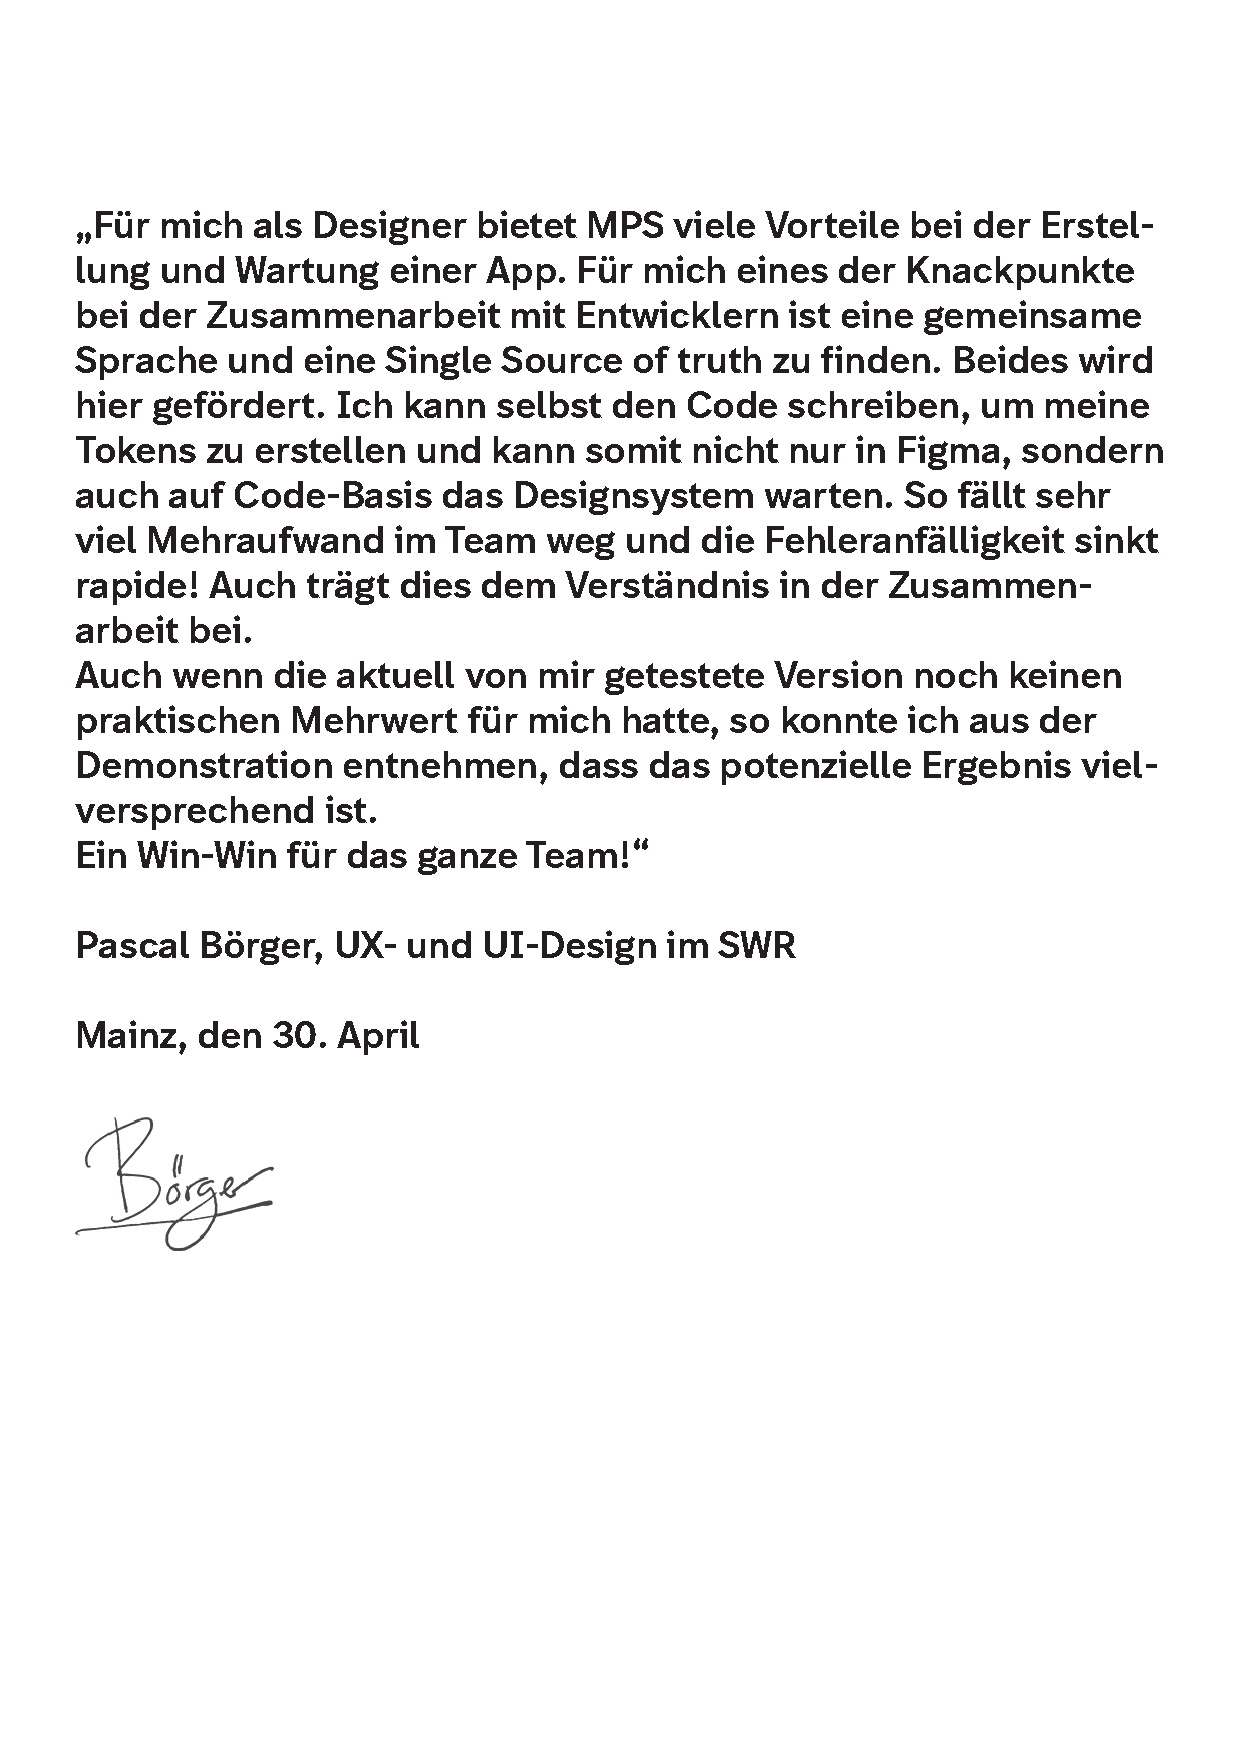
\includepdf[addtotoc={1,subsubsection,1,Pascal Börger,appendix:pascal-borger},pagecommand={}]{../assets/appendix/feedback_pb}

\includepdf[addtotoc={1,subsubsection,1,Julian Hültenschmidt,appendix:julian-hultenschmidt},pagecommand={}]{../assets/appendix/feedback_jh}

\includepdf[addtotoc={1,subsubsection,1,Bayram Ünlü,appendix:bayram-unlu},pagecommand={}]{../assets/appendix/feedback_jh}

\subsection{Eidesstattliche Versicherung}\label{appendix:eidesstattliche-versicherung}
Hiermit versichere ich an Eides statt, dass ich die vorliegende Bachelorarbeit mit dem Titel \enquote{\thetitle} selbstständig und ohne Hilfe Dritter verfasst habe.
Ich habe keine anderen als die angegebenen Hilfsmittel und Quellen benutzt.
Alle wörtlich oder sinngemäß übernommenen Textstellen habe ich als solche kenntlich gemacht.
Ich versichere, dass ich die Arbeit in dieser oder einer ähnlichen Form noch keiner anderen Prüfungsbehörde vorgelegt habe.
Mir ist bekannt, dass bei einem Verstoß gegen diese Grundsätze die Arbeit als nicht bestanden bewertet werden kann.

\vfill

\noindent Ort, Datum: Dorsten, \today \hspace{1cm} Unterschrift: \hrulefill           \\
\phantom{Ort, Datum: Dorsten, \today \hspace{1cm} Unterschrift:} \theauthor

\end{document}
